 
%%% DOCUMENTCLASS 
%%%-------------------------------------------------------------------------------

\documentclass[
a4paper, % Stock and paper size.
10pt, % Type size.
% article,
% oneside, 
onecolumn, % Only one column of text on a page.
% openright, % Each chapter will start on a recto page.
% openleft, % Each chapter will start on a verso page.
openany, % A chapter may start on either a recto or verso page.
]{memoir}

%%% PACKAGES 
%%%------------------------------------------------------------------------------
\usepackage[utf8x]{inputenc} % If utf8 encoding
% \usepackage[lantin1]{inputenc} % If not utf8 encoding, then this is probably the way to go
\usepackage[T1]{fontenc}    %
\usepackage[english]{babel} % English please
\usepackage[final]{microtype} % Less badboxes
% \usepackage{kpfonts} %Font
\usepackage{amsmath,amssymb,mathtools} % Math
% \usepackage{tikz} % Figures
\usepackage{graphicx} % Include figures
\usepackage{listings}    % Add code snippets
\usepackage[usenames,dvipsnames,svgnames,table]{xcolor}
\usepackage[linktocpage=true]{hyperref} % Extensive support for hypertext in LaTeX
\usepackage[usenames,dvipsnames]{xcolor} %used for font color
\usepackage{dirtree} % Make directory trees easily
\usepackage{framed} % shade in a region of the page
\usepackage{multirow}  % use rows spanning multiple columns in tables
\usepackage{float}
\usepackage[all]{background}
\usepackage[most]{tcolorbox}

%%% PAGE LAYOUT 
%%%------------------------------------------------------------------------------

\setlrmarginsandblock{0.15\paperwidth}{*}{1} % Left and right margin
\setulmarginsandblock{0.2\paperwidth}{*}{1}  % Upper and lower margin
\checkandfixthelayout

%%% SECTIONAL DIVISIONS
%%%------------------------------------------------------------------------------

\maxsecnumdepth{subsubsection} % Subsections (and higher) are numbered
\setsecnumdepth{subsubsection}

\makeatletter %
\makechapterstyle{standard}{
  \setlength{\beforechapskip}{0\baselineskip}
  \setlength{\midchapskip}{1\baselineskip}
  \setlength{\afterchapskip}{2\baselineskip}
  \renewcommand{\chapterheadstart}{\vspace*{\beforechapskip}}
  \renewcommand{\chapnamefont}{\centering\normalfont\huge}
  \renewcommand{\printchaptername}{\chapnamefont \@chapapp}
  \renewcommand{\chapternamenum}{\space}
  \renewcommand{\chapnumfont}{\normalfont\huge}
  \renewcommand{\printchapternum}{\chapnumfont \thechapter}
  \renewcommand{\afterchapternum}{\par\nobreak\vskip \midchapskip}
  \renewcommand{\printchapternonum}{\vspace*{\midchapskip}\vspace*{5mm}}
  \renewcommand{\chaptitlefont}{\centering\bfseries\HUGE}
  \renewcommand{\printchaptertitle}[1]{\chaptitlefont ##1}
  \renewcommand{\afterchaptertitle}{\par\nobreak\vskip \afterchapskip}
}
\makeatother

\chapterstyle{standard}

\setsecheadstyle{\normalfont\huge\bfseries}
\setsubsecheadstyle{\normalfont\large\bfseries}
\setparaheadstyle{\normalfont\normalsize\bfseries}
\setparaindent{0pt}\setafterparaskip{0pt}

%%% FLOATS AND CAPTIONS
%%%------------------------------------------------------------------------------

\makeatletter                  % You do not need to write [htpb] all the time
\renewcommand\fps@figure{htbp} %
\renewcommand\fps@table{htbp}  %
\makeatother                   %

\captiondelim{\space } % A space between caption name and text
\captionnamefont{\small\bfseries} % Font of the caption name
\captiontitlefont{\small\normalfont} % Font of the caption text

\changecaptionwidth          % Change the width of the caption
\captionwidth{1\textwidth} %

%%% ABSTRACT
%%%------------------------------------------------------------------------------

\renewcommand{\abstractnamefont}{\normalfont\small\bfseries} % Font of abstract title
\setlength{\absleftindent}{0.1\textwidth} % Width of abstract
\setlength{\absrightindent}{\absleftindent}

%%% HEADER AND FOOTER 
%%%------------------------------------------------------------------------------

\makepagestyle{standard} % Make standard pagestyle

\makeatletter                 % Define standard pagestyle
\makeevenfoot{standard}{}{}{} %
\makeoddfoot{standard}{}{}{}  %
\makeevenhead{standard}{\bfseries\thepage\normalfont\qquad\small\leftmark}{}{}
\makeoddhead{standard}{}{}{\small\rightmark\qquad\bfseries\thepage}
% \makeheadrule{standard}{\textwidth}{\normalrulethickness}
\makeatother                  %

\makeatletter
\makepsmarks{standard}{
\createmark{chapter}{both}{shownumber}{\@chapapp\ }{ \quad }
\createmark{section}{right}{shownumber}{}{ \quad }
\createplainmark{toc}{both}{\contentsname}
\createplainmark{lof}{both}{\listfigurename}
\createplainmark{lot}{both}{\listtablename}
\createplainmark{bib}{both}{\bibname}
\createplainmark{index}{both}{\indexname}
\createplainmark{glossary}{both}{\glossaryname}
}
\makeatother                               %

\makepagestyle{chap} % Make new chapter pagestyle

\makeatletter
\makeevenfoot{chap}{}{\small\bfseries\thepage}{} % Define new chapter pagestyle
\makeoddfoot{chap}{}{\small\bfseries\thepage}{}  %
\makeevenhead{chap}{}{}{}   %
\makeoddhead{chap}{}{}{}    %
% \makeheadrule{chap}{\textwidth}{\normalrulethickness}
\makeatother

\nouppercaseheads
\pagestyle{standard}               % Choosing pagestyle and chapter pagestyle
\aliaspagestyle{chapter}{chap} %

%%% NEW COMMANDS
%%%------------------------------------------------------------------------------
% custom commands defined in here (must be called before constants)
%%%%%%%%%%%%%%%%%%%%%%%%%%%%%%%%%%%%%%%%%%%%%%%%%%%%%%%%
%%
%%  New colours
%%
%%%%%%%%%%%%%%%%%%%%%%%%%%%%%%%%%%%%%%%%%%%%%%%%%%%%%%%%

\definecolor{codegreen}{rgb}{0,0.6,0}
\definecolor{codegray}{rgb}{0.5,0.5,0.5}
\definecolor{codepurple}{rgb}{0.58,0,0.82}
\definecolor{darkgray}{rgb}{0.20,0.20,0.20}
\definecolor{backcolour1}{rgb}{0.95,0.95,0.92}
\definecolor{backcolour2}{rgb}{1,0.977,0.801}
\definecolor{backcolour3}{rgb}{0.79,0.88,1}


%%%%%%%%%%%%%%%%%%%%%%%%%%%%%%%%%%%%%%%%%%%%%%%%%%%%%%%%
%%
%%  formatting constants
%%
%%%%%%%%%%%%%%%%%%%%%%%%%%%%%%%%%%%%%%%%%%%%%%%%%%%%%%%%

% formatting the named variables (from user setup)
\newcommand{\definevariable}[1]{\textcolor{blue}{\{#1\}}}
\newcommand{\definevariablecmd}[1]{\textcolor{cyan}{\{#1\}}}

% --------------------------------------------------------
% formatting the named keywords 
\newcommand{\definekeyword}[1]{\textcolor{red}{\{#1\}}}

% --------------------------------------------------------
% Program should be in small caps
\newcommand{\Program}[1]{\textsc{#1}}

% --------------------------------------------------------
% Double underscore
\newlength\dunder
\settowidth{\dunder}{\_}
\newcommand{\twound}{\rule{1.25\dunder}{0.2pt}}

% --------------------------------------------------------
% formatting for the directories trees
\newcommand{\customdirtree}[1]{
\renewcommand*\DTstylecomment{\ttfamily\textcolor{black}}
\renewcommand*\DTstyle{\ttfamily\textcolor{blue}}
\dirtree{%
#1}
}

% --------------------------------------------------------
% Parameters
% \ParameterEntry{Name}{Description}{variable}{default value}{used in}{location}{level (if dev)}
\newcommand{\ParameterEntry}[8]{
	\begin{minipage}[t]{\textwidth}
	\textbf{#1 (\textcolor{red}{#3})}

	\begin{thighlight}
	\textcolor{brown}{#2} 

	\begin{tabular}{>{\color{red}}l c l}
	&&\\
	#3 & = & #4 \\
	&&\\
	\textcolor{blue}{Used in:}  & \multicolumn{2}{p{10cm}}{#5} \\
	\textcolor{blue}{Defined in:} & \multicolumn{2}{p{10cm}}{#6} \\
	\ifdevguide
	\textcolor{blue}{Called in:} & \multicolumn{2}{p{10cm}}{\textcolor{codegreen}{#7}} \\
	\textcolor{blue}{Level:} & \multicolumn{2}{p{10cm}}{#8} \\
	\fi
	\end{tabular}
	\end{thighlight}
	\end{minipage}
}


\newcommand{\PseudoParamEntry}[7]{
	\begin{minipage}[t]{\textwidth}
	\textbf{#1 (\textcolor{red}{#3})}

	\begin{thighlight}
	\textcolor{codegreen}{#2} 

	\begin{tabular}{>{\color{red}}l c l}
	&&\\
	#3 && \\
	&&\\
	\textcolor{blue}{Used in:}  & \multicolumn{2}{p{10cm}}{#4} \\
	\textcolor{blue}{Defined in:} & \multicolumn{2}{p{10cm}}{#5} \\
	\ifdevguide
	\textcolor{blue}{Called in:} & \multicolumn{2}{p{10cm}}{\textcolor{codegreen}{#6}} \\
	\textcolor{blue}{Level:} & \multicolumn{2}{p{10cm}}{#7} \\
	\fi
	\end{tabular}
	\end{thighlight}
	\end{minipage}
}


% --------------------------------------------------------
% define dev sections notes etc

\newcommand{\devsection}[2]{
\ifdevguide
\section{#1}

#2
\fi
}


\newcommand{\DevNote}[1]{
\ifdevguide
\begin{note}
#1
\end{note}
\fi
}
% get code highlighting parameters

\lstdefinestyle{text}{
    commentstyle=\color{codegreen},
    keywordstyle=\color{magenta},
    numberstyle=\tiny\color{codegray},
    stringstyle=\color{codepurple},
    basicstyle=\linespread{1.2}\ttfamily\footnotesize,
    breakatwhitespace=false,         
    breaklines=true,                 
    captionpos=b,                    
    keepspaces=true,                 
    % numbers=left,                    
    % numbersep=5pt,                  
    showspaces=false,                
    showstringspaces=false,
    showtabs=false,                  
    tabsize=2,
    moredelim=**[is][\color{red}]{@}{@},
    moredelim=**[is][\color{OliveGreen}]{<}{>},
    extendedchars=false,
    columns=fullflexible,
    escapeinside={(*}{*)},%
	  literate={\\@}{{\unichar{"0040}}}1
			 {\\<}{{\unichar{"003C}}}1 
			 {\\>}{{\unichar{"003E}}}1
}

\lstdefinestyle{bashstyle}{
	language=bash,  
    commentstyle=\color{codegreen},
    keywordstyle=\color{magenta},
    numberstyle=\tiny\color{codegray},
    stringstyle=\color{codepurple},
    basicstyle=\linespread{1.2}\ttfamily\footnotesize,
    breakatwhitespace=false,         
    breaklines=true,                 
    captionpos=b,                    
    keepspaces=true,                 
    % numbers=left,                    
    % numbersep=5pt,                  
    showspaces=false,                
    showstringspaces=false,
    showtabs=false,                  
    tabsize=2,
    moredelim=**[is][\color{red}]{@}{@},
    moredelim=**[is][\color{OliveGreen}]{<}{>},
    extendedchars=false,
    columns=fullflexible,
    escapeinside={(*}{*)},%
    literate={\\@}{{\unichar{"0040}}}1
       {\\<}{{\unichar{"003C}}}1 
       {\\>}{{\unichar{"003E}}}1
}


\lstdefinestyle{cshstyle}{
  language=sh,  
    commentstyle=\color{codegreen},
    keywordstyle=\color{magenta},
    numberstyle=\tiny\color{codegray},
    stringstyle=\color{codepurple},
    basicstyle=\linespread{1.2}\ttfamily\footnotesize,
    breakatwhitespace=false,         
    breaklines=true,                 
    captionpos=b,                    
    keepspaces=true,                 
    % numbers=left,                    
    % numbersep=5pt,                  
    showspaces=false,                
    showstringspaces=false,
    showtabs=false,                  
    tabsize=2,
    moredelim=**[is][\color{red}]{@}{@},
    moredelim=**[is][\color{OliveGreen}]{<}{>},
    extendedchars=false,
    columns=fullflexible,
    escapeinside={(*}{*)},%
    literate={\\@}{{\unichar{"0040}}}1
       {\\<}{{\unichar{"003C}}}1 
       {\\>}{{\unichar{"003E}}}1
}

\lstdefinestyle{cmdstyle}{
    language=command.com,
    commentstyle=\color{codegreen},
    keywordstyle=\color{blue!35!white},
    numberstyle=\tiny\color{codegray},
    stringstyle=\color{codepurple},
    basicstyle=\linespread{1.2}\ttfamily\footnotesize\color{white},
    breakatwhitespace=false,         
    breaklines=true,                 
    captionpos=b,                    
    keepspaces=true,                 
    % numbers=left,                    
    % numbersep=5pt,                  
    showspaces=false,                
    showstringspaces=false,
    showtabs=false,                  
    tabsize=2,
    extendedchars=false,
    columns=fullflexible,
    morekeywords={chmod, unzip},
    escapeinside={(*}{*)},%
}

\lstdefinestyle{cmdstyleprint}{
    commentstyle=\color{codegreen},
    keywordstyle=\color{blue!35!white},
    numberstyle=\tiny\color{codegray},
    stringstyle=\color{codepurple},
    basicstyle=\linespread{1.2}\ttfamily\footnotesize\color{white},
    breakatwhitespace=false,         
    breaklines=true,                 
    captionpos=b,                    
    keepspaces=true,                 
    % numbers=left,                    
    % numbersep=5pt,                  
    showspaces=false,                
    showstringspaces=false,
    showtabs=false,                  
    tabsize=2,
    extendedchars=false,
    columns=fullflexible,
    morekeywords={chmod, unzip},
    escapeinside={(*}{*)},%
}

\lstdefinestyle{pythonstyle}{
    language=Python,
    commentstyle=\color{codegreen},
    keywordstyle=\color{magenta},
    numberstyle=\tiny\color{codegray},
    stringstyle=\color{codepurple},
    basicstyle=\linespread{1.2}\ttfamily\footnotesize,
    breakatwhitespace=false,         
    breaklines=true,                 
    captionpos=b,                    
    keepspaces=true,                 
    % numbers=left,                    
    % numbersep=5pt,                  
    showspaces=false,                
    showstringspaces=false,
    showtabs=false,                  
    tabsize=2,
    moredelim=**[is][\color{red}]{@}{@},
    extendedchars=false,
    columns=fullflexible,
    escapeinside={(*}{*)},%
    literate={\\@}{{\unichar{"0040}}}1
}


\lstdefinestyle{pythoninline}{
    language=Python,
    backgroundcolor=\color{backcolour3},   
    commentstyle=\color{codegreen},
    keywordstyle=\color{magenta},
    numberstyle=\tiny\color{codegray},
    stringstyle=\color{codepurple},
    basicstyle=\ttfamily\scriptsize,
    breakatwhitespace=false,         
    breaklines=true,                 
    captionpos=b,                    
    keepspaces=true,                 
    % numbers=left,                    
    % numbersep=5pt,                  
    showspaces=false,                
    showstringspaces=false,
    showtabs=false,                  
    tabsize=2,
    moredelim=**[is][\color{red}]{@}{@},
    extendedchars=false,
    columns=fullflexible,
    literate={\\@}{{\unichar{"0040}}}1
}

\tcbuselibrary{listings}
\tcbuselibrary{breakable}

% example:
% \newtcblisting{mylisting}{
%       arc=0pt,
%       top=0mm,
%       bottom=0mm,
%       left=0mm,
%       right=0mm,
%       boxrule=0pt,
%       colback=black,
%       listing only,
%       listing options={style=mystyle},
%       hbox
% }


\newtcblisting{textbox}{
      before skip=3pt,
      after skip=6pt,
      %tcbox raise base,
      top=0pt,bottom=0pt,left=0mm,right=0mm,
      %toprule=0.3mm,bottomrule=0.3mm,boxsep=0.5mm,
      colback=backcolour1,
      colframe=backcolour1!75!black,
      fonttitle={\tiny\bfseries},
      title={text},  % Fixed title
      listing only,
      listing options={style=text},
}

\newtcblisting{bashbox}{
      before skip=3pt,
      after skip=6pt,
      %tcbox raise base,
      top=0pt,bottom=0pt,left=2mm,right=0mm,
      %toprule=0.3mm,bottomrule=0.3mm,boxsep=0.5mm,
      colback=backcolour1,
      colframe=backcolour1!75!black,
      fonttitle={\tiny\bfseries},
      title={bash},  % Fixed title
      listing only,
      listing options={style=bashstyle},
}

\newtcblisting{cshbox}{
      before skip=3pt,
      after skip=6pt,
      %tcbox raise base,
      top=0pt,bottom=0pt,left=0mm,right=0mm,
      %toprule=0.3mm,bottomrule=0.3mm,boxsep=0.5mm,
      colback=backcolour1,
      colframe=backcolour1!75!black,
      fonttitle={\tiny\bfseries},
      title={tcsh/csh},  % Fixed title
      listing only,
      listing options={style=cshstyle},
}

\newtcblisting{cmdbox}{
      before skip=3pt,
      after skip=6pt,
      %tcbox raise base,
      top=0pt,bottom=0pt,left=2mm,right=0mm,
      %toprule=0.3mm,bottomrule=0.3mm,boxsep=0.5mm,
      colback=darkgray,
      colframe=darkgray!75!black,
      fonttitle={\tiny\bfseries},
      title={CMD input},  % Fixed title
      listing only,
      listing options={style=cmdstyle},
      every listing line={\textcolor{red}{\small\ttfamily\bfseries \textgreater{\textgreater}\,\,\,}}
}

\newtcblisting{cmdboxprint}{
      before skip=3pt,
      after skip=6pt,
      %tcbox raise base,
      top=0pt,bottom=0pt,left=2mm,right=0mm,
      %toprule=0.3mm,bottomrule=0.3mm,boxsep=0.5mm,
      colback=darkgray,
      colframe=darkgray!75!black,
      fonttitle={\tiny\bfseries},
      title={Command line output},  % Fixed title
      listing only,
      listing options={style=cmdstyleprint}
}

\newtcblisting{pythonbox}{
      before skip=3pt,
      after skip=6pt,
      %tcbox raise base,
      top=0pt,bottom=0pt,left=2mm,right=0mm,
      %toprule=0.3mm,bottomrule=0.3mm,boxsep=0.5mm,
      colback=backcolour3,
      colframe=backcolour3!75!black,
      fonttitle={\tiny\bfseries},
      title={Python/Ipython},  % Fixed title
      listing only,
      listing options={style=pythonstyle},
}

\newtcolorbox{note}[1][]{%
  enhanced jigsaw, % better frame drawing
  borderline west={2pt}{0pt}{red}, % straigh vertical line at the left edge
  sharp corners, % No rounded corners
  boxrule=0pt, % no real frame,
  fonttitle={\large\bfseries},
  coltitle={black},  % Black colour for title
  title={Note:\ },  % Fixed title
  attach title to upper, % Move the title into the box
  #1
}

\newtcolorbox{todo}[1][]{%
  enhanced jigsaw, % better frame drawing
  borderline west={2pt}{0pt}{green}, % straigh vertical line at the left edge
  sharp corners, % No rounded corners
  boxrule=0pt, % no real frame,
  fonttitle={\large\bfseries},
  coltitle={black},  % Black colour for title
  title={TODO:\ },  % Fixed title
  attach title to upper, % Move the title into the box
  #1
}


\newtcolorbox{thighlight}[1][]{%
  enhanced jigsaw, % better frame drawing
  before skip=3pt,
  after skip=6pt,
  borderline west={2pt}{0pt}{orange}, % straigh vertical line at the left edge
  sharp corners, % No rounded corners
  boxrule=0pt, % no real frame,
  colback=yellow!10!white,
  attach title to upper, % Move the title into the box
  {#1}
}

\newtcolorbox{tcustomdir}[1][]{%
  enhanced jigsaw, % better frame drawing
  before skip=3pt,
  after skip=6pt,
  borderline west={2pt}{0pt}{blue}, % straigh vertical line at the left edge
  %sharp corners, % No rounded corners
  boxrule=0pt, % no real frame,
  colback=blue!10!white,
  attach title to upper, % Move the title into the box
  #1
}


\newtcblisting{pythonboxblank}{
      before skip=3pt,
      after skip=6pt,
      %tcbox raise base,
      top=0pt,bottom=0pt,left=2mm,right=0mm,
      %toprule=0.3mm,bottomrule=0.3mm,boxsep=0.5mm,
      listing only,
      listing options={style=pythonstyle},
}
% custom constants defined in here
% ----------------------------------------------
% Program constants that can be changed through-out the document

% ----------------------------------------------
% Manual version, authors and dates
% ----------------------------------------------
% the current versions of the manuals
\newcommand{\MyVersion}{0.3.003}
\newcommand{\MyVersionUser}{\MyVersion}
\newcommand{\MyVersionDev}{\MyVersion}

% the last date modified for the manuals
\newcommand{\MyDate}{2018-06-29}
\newcommand{\MyDateUser}{\MyDate}
\newcommand{\MyDateDev}{\MyDate}

% the author list of the manuals
\newcommand{\MyAuthors}{N. Cook, F. Bouchy, E. Artigau, , M. Hobson, C. Moutou, I. Boisse, E. Martioli}

% the id of the manuals
\newcommand{\MyID}{SPIROU-4800-LAM-UM-00961}
\newcommand{\MyIDuser}{\MyID}
\newcommand{\MyIDdev}{\MyID}
% ----------------------------------------------
% DRS variables
% ----------------------------------------------
% The version of the DRS code
\newcommand{\MyCodeVersion}{0.2.056 (alpha pre-release)}

% The instrument
\newcommand{\instrument}{SPIRou\,}

% The latest download links
\newcommand{\DRSLatestURL}{https://github.com/njcuk9999/spirou\_py3\,}

\newcommand{\DRSGitURL}{https://github.com/njcuk9999/spirou\_py3.git\,}

\newcommand{\DRSsshURL}{git@github.com:njcuk9999/spirou\_py3.git\,}

% ----------------------------------------------
% Commonly used variables
% ----------------------------------------------

% short cuts to the recipe names
\newcommand{\calDARK}{\definevariable{ch:the_recipes:cal_DARK_spirou}{cal\_DARK\_spirou}\,}

\newcommand{\calDRIFTRAW}{\definevariable{ch:the_recipes:cal_DRIFT_RAW_spirou}{cal\_DRIFT\_RAW\_spirou}\,}

\newcommand{\calDRIFTE}{\definevariable{ch:the_recipes:cal_DRIFT_RAW_spirou}{cal\_DRIFT\_E2DS\_spirou}\,}

\newcommand{\calDRIFTPEAK}{\definevariable{ch:the_recipes:cal_DRIFT_RAW_spirou}{cal\_DRIFTPEAK\_E2DS\_spirou}\,}

\newcommand{\calextractRAW}{\definevariable{ch:the_recipes:cal_extract_RAW_spirou}{cal\_extract\_RAW{\hskip 0pt}\_spirou}\,}

\newcommand{\calextractRAWALL}{\definevariable{ch:the_recipes:cal_extract_RAW_spirou}{cal\_extract\_RAW{\hskip 0pt}\_spirouALL}\,}

\newcommand{\calextractRAWAB}{\definevariable{ch:the_recipes:cal_extract_RAW_spirou}{cal\_extract\_RAW{\hskip 0pt}\_spirouAB}\,}

\newcommand{\calextractRAWC}{\definevariable{ch:the_recipes:cal_extract_RAW_spirou}{cal\_extract\_RAW{\hskip 0pt}\_spirouC}\,}

\newcommand{\calFFraw}{\definevariable{ch:the_recipes:cal_FF_RAW_spirou}{cal\_FF\_RAW\_spirou}\,}

\newcommand{\callocRAW}{\definevariable{ch:the_recipes:cal_loc_RAW_spirou}{cal\_loc\_RAW\_spirou}\,}

\newcommand{\calSLIT}{\definevariable{ch:the_recipes:cal_SLIT_spirou}{cal\_SLIT\_spirou}\,}

\newcommand{\calbadpix}{\definevariable{ch:the_recipes:cal_BADPIX_spirou}{cal\_BADPIX\_spirou}\,}

\newcommand{\calCCF}{\definevariable{ch:the_recipes:cal_CCF_E2DS_spirou}{cal\_CCF\_E2DS\_spirou}\,}

\newcommand{\calWAVE}{\definevariable{ch:the_recipes:cal_WAVE_E2DS_spirou}{cal\_WAVE\_E2DS\_spirou}\,}

\newcommand{\calHC}{\definevariable{ch:the_recipes:cal_HC_E2DS_spirou}{cal\_HC\_E2DS\_spirou}\,}

\newcommand{\polspirou}{\definevariable{ch:the_recipes:pol_spirou}{pol\_spirou}\,}

\newcommand{\calpreprocess}{\definevariable{ch:the_recipes}{cal\_preprocess\_spirou}\,}

\newcommand{\calexometer}{\definevariable{ch:the_recipes}{cal\_exposure\_meter}\,}

\newcommand{\offlisting}{\definevariable{ch:the_recipes}{off\_listing\_RAW\_spioru}\,}

\newcommand{\visuEDS}{\definevariable{ch:the_recipes}{visu\_E2DS\_spirou}\,}

\newcommand{\visuRAW}{\definevariable{ch:the_recipes}{visu\_RAW\_spirou}\,}

\newcommand{\visuWAVE}{\definevariable{ch:the_recipes}{visu\_WAVE\_spirou}\,}

\newcommand{\calvalidate}{\definevariable{ch:the_recipes:cal_validate_spirou}{cal\_validate\_spirou}\,}

% Define all recipes
\newcommand{\AllRecipes}{All Recipes\,}

% Define modules
\newcommand{\progMAIN}{\textcolor{blue}{main()}\,}

\newcommand{\spirouBACK}{\definevariable{ch:the_module:spirouBACK}{SpirouDRS{\hskip 0pt}.spirouBACK{\hskip 0pt}.spirouBACK}\,}

\newcommand{\spirouCDB}{\definevariable{ch:the_module:spirouCDB}{SpirouDRS{\hskip 0pt}.spirouCDB{\hskip 0pt}.spirouCDB}\,}

\newcommand{\spirouConfig}{\definevariable{ch:the_module:spirouConfig}{SpirouDRS{\hskip 0pt}.spirouConfig{\hskip 0pt}.spirouConfig}\,}

\newcommand{\spirouConst}{\definevariable{ch:the_module:spirouConfig}{SpirouDRS{\hskip 0pt}.spirouConfig{\hskip 0pt}.spirouConst}\,}

\newcommand{\spirouCore}{\definevariable{ch:the_module:spirouCore}{SpirouDRS{\hskip 0pt}.spirouCore{\hskip 0pt}.spirouCore}\,}

\newcommand{\spirouLog}{\definevariable{ch:the_module:spirouCore}{SpirouDRS{\hskip 0pt}.spirouCore{\hskip 0pt}.spirouLog}\,}

\newcommand{\spirouPlot}{\definevariable{ch:the_module:spirouCore}{SpirouDRS{\hskip 0pt}.spirouCore{\hskip 0pt}.spirouPlot}\,}

\newcommand{\spirouEXTOR}{\definevariable{ch:the_module:spirouEXTOR}{SpirouDRS{\hskip 0pt}.spirouEXTOR{\hskip 0pt}.spirouEXTOR}\,}

\newcommand{\spirouFLAT}{\definevariable{ch:the_module:spirouFLAT}{SpirouDRS{\hskip 0pt}.spirouFLAT{\hskip 0pt}.spirouFLAT}\,}

\newcommand{\spirouFITS}{\definevariable{ch:the_module:spirouImage}{SpirouDRS{\hskip 0pt}.spirouImage{\hskip 0pt}.spirouFITS}\,}

\newcommand{\spirouImage}{\definevariable{ch:the_module:spirouImage}{SpirouDRS{\hskip 0pt}.spirouImage{\hskip 0pt}.spirouImage}\,}

\newcommand{\spirouFile}{\definevariable{ch:the_module:spirouImage}{SpirouDRS{\hskip 0pt}.spirouImage{\hskip 0pt}.spirouFile}\,}

\newcommand{\spirouExposeMeter}{\definevariable{ch:the_module:spirouImage}{SpirouDRS{\hskip 0pt}.spirouImage{\hskip 0pt}.spirouExposeMeter}\,}

\newcommand{\spirouLOCOR}{\definevariable{ch:the_module:spirouLOCOR}{SpirouDRS{\hskip 0pt}.spirouLOCOR{\hskip 0pt}.spirouLOCOR}\,}

\newcommand{\spirouRV}{\definevariable{ch:the_module:spirouRV}{SpirouDRS{\hskip 0pt}.spirouRV{\hskip 0pt}.spirouRV}\,}

\newcommand{\spirouStartup}{\definevariable{ch:the_module:spirouStartup}{SpirouDRS{\hskip 0pt}.spirouStartup{\hskip 0pt}.spirouStartup}\,}

\newcommand{\spirouTHORCA}{\definevariable{ch:the_module:spirouTHORCA}{SpirouDRS{\hskip 0pt}.spirouTHORCA{\hskip 0pt}.spirouTHORCA}\,}

\newcommand{\spirouWAVE}{\definevariable{ch:the_module:spirouTHORCA}{SpirouDRS{\hskip 0pt}.spirouTHORCA{\hskip 0pt}.spirouWAVE}\,}

\newcommand{\spirouPOLAR}{\definevariable{ch:the_module:spirouPOLAR}{SpirouDRS{\hskip 0pt}.spirouPOLAR{\hskip 0pt}.spirouPOLAR}\,}

% python specifics
\newcommand{\MAIN}{\twound{main}\twound{()}\,}

\newcommand{\INIT}{\twound{init}\twound{()}\,}

\newcommand{\WLOG}{\definevariable{ch:the_module:spirouCore:logger}{WLOG}\,}

\newcommand{\ParamDict}{\definevariable{ch:the_module:spirouConfig:ParamDict}{ParamDict}\,}

\newcommand{\ConfigError}{\definevariable{ch:the_module:spirouConfig:ConfigError}{ConfigError}\,}

% variable the user should identify with their installation directory
\newcommand{\InstallDIR}{\definevariable{text:drs_root}{DRS\_ROOT}\,}

\newcommand{\reduceddir}{\definevariable{text:reduced_dir}{reduced\_dir}\,}

\newcommand{\argnightname}{\definevariable{text:arg_night_name}{arg\_night\_name}\,}

\newcommand{\argfilenames}{\definevariable{text:arg_file_names}{arg\_file\_names}\,}

\newcommand{\calibdb}{\definevariable{ch:data_architecture:calibDB}{calibration database}\,}

% keyword commands
\newcommand{\rootdrsloc}{\defineoutkeyword{text:root_drs_loc}{kw\_root\_drs\_loc}\,}

\newcommand{\rootdrsflat}{\defineoutkeyword{text:root_drs_flat}{kw\_root\_drs\_flat}\,}

% name for mac operating system
\newcommand{\mac}{macOS\,}

% name of the master calibDB file
\newcommand{\masterCALIBDBfile}{\definevariable{text:ic_calibDB_filename}{ic\_calibDB\_filename}\,}

% name of the config directory
\newcommand{\configdir}{config\,}
\newcommand{\configdirrelpath}{../\configdir\,}
% name of the main config file
\newcommand{\configtxtfile}{\configdirrelpath/config.py\,}
\newcommand{\configtxtfilerelpath}{\configtxtfile}
\newcommand{\configtxtfilepath}{\InstallDIR/{\hskip 0pt}\configdir/{\hskip 0pt}\configtxtfile}
% name of the user constants file
\newcommand{\constantsfile}{constants\_SPIROU\_H4RG.py}
\newcommand{\constantsfilepath}{\InstallDIR/{\hskip 0pt}\configdir/{\hskip 0pt}\constantsfile}
% name of the spirou constants file
\newcommand{\spirouCONST}{SpirouDRS.spirouConfig{\hskip 0pt}.spirouConst\,}
% name of the spirou keywords file
\newcommand{\spirouKeywords}{SpirouDRS.spirouConfig{\hskip 0pt}.spirouKeywords\,}
% This sets the header value for the time in calibDB
\newcommand{\constantAcqtimeKey}{ACQTIME1\,}
% This sets the folder name date format
\newcommand{\constantFolderDateFormat}{YYYYMMDD\,}

% Not mine
\newcommand{\p}{\partial} %Partial
% Or what ever you want


%%% MARGIN
%%%------------------------------------------------------------------------------
\SetBgContents{\MyIDuser}% Set contents
\SetBgPosition{-0.75cm,-0.3\textheight}% Select location
\SetBgOpacity{1.0}% Select opacity
\SetBgAngle{90.0}% Select rotation of logo
\SetBgScale{1.25}% Select scale factor of logo

%%% TABLE OF CONTENTS
%%%------------------------------------------------------------------------------

\maxtocdepth{subsection} % Only parts, chapters and sections in the table of contents
\settocdepth{subsection}

% \maxtocdepth{section} % Only parts, chapters and sections in the table of contents
% \settocdepth{section}

\AtEndDocument{\addtocontents{toc}{\par}} % Add a \par to the end of the TOC

\renewcommand*{\cftappendixname}{Appendix\space}

%%% INTERNAL HYPERLINKS
%%%-------------------------------------------------------------------------------

\usepackage{hyperref}   % Internal hyperlinks
\hypersetup{
    pdfauthor={Neil James Cook},
    pdfcreator={Neil James Cook},
    pdftitle={SPIRou User Guide},
    pdfsubject={SPIRou DRS},
    pdfkeywords={SPIRou, DRS, Pipeline},
    colorlinks=true,         % false: boxed links; true: colored links
    linkcolor=blue,          % color of internal links (change box color with linkbordercolor)
    citecolor=Maroon,        % color of links to bibliography
    filecolor=blue,          % color of file links
    urlcolor=blue,           % color of external links
    plainpages=false,       
}
\usepackage{memhfixc}   %



%%% THE DOCUMENT
%%% Where all the important stuff is included!
%%%-------------------------------------------------------------------------------

\author{\MyAuthors}
\title{{\Huge SPIRou Data Reduction Software} \vspace{1cm} \\ \HUGE{User Guide} \\ {\small \MyVersionUser} \\ For DRS \instrument \MyCodeVersion}
\date{\MyDateUser}

% \usepackage{lipsum} % Just to put in some text

\begin{document}

\frontmatter

\maketitle

% Add logo to title page
\vspace{1cm}
\begin{center}

\includegraphics[width=.5\textwidth]{Figures/Logo_SPIRou-22.pdf}
\end{center}
\vspace{1cm}

\begin{abstract}
\noindent This is the guide to installing, running, and using the SPIRou DRS. 
\end{abstract}
\clearpage

\tableofcontents*
\clearpage

% Introduction
%%%%%%%%%%%%%%%%%%%%%%%%%%%%%%%%%%%%%%%%%%%%%%%%%%%%%%%%
%%
\chapter{Introduction}
\label{chapter:introduction}
%%
%%%%%%%%%%%%%%%%%%%%%%%%%%%%%%%%%%%%%%%%%%%%%%%%%%%%%%%%


%%%-------------------------------------------------------------------------------
\mainmatter
% Define the chapters here
%%%-------------------------------------------------------------------------------

% Chapter 1: Installation guide
%%%%%%%%%%%%%%%%%%%%%%%%%%%%%%%%%%%%%%%%%%%%%%%%%%%%%%%%
%%
\chapter{Installation}
\label{chapter:installation}
%%
%%%%%%%%%%%%%%%%%%%%%%%%%%%%%%%%%%%%%%%%%%%%%%%%%%%%%%%%


%%%%%%%%%%%%%%%%%%%%%%%%%%%%%%%%%%%%%%%%%%%%%%%%%%%%%%%%
%%
\section{Introduction}
\label{ch:install:installintro}
%%
%%%%%%%%%%%%%%%%%%%%%%%%%%%%%%%%%%%%%%%%%%%%%%%%%%%%%%%%

Once finalized the installation should just be a download, run setup.py and configure the DRS directories, however, during development the following stages are required.

\DevNote{Currently the download repository on git-hub is private and requires a git-hub account, and the user to be added to the list of collaborators. To be added to the collaborators please email \url{neil.james.cook@gmail.com} with your git-hub user name.}







%%%%%%%%%%%%%%%%%%%%%%%%%%%%%%%%%%%%%%%%%%%%%%%%%%%%%%%%
%%
\section{Download}
\label{ch:install:installDownload}
%%
%%%%%%%%%%%%%%%%%%%%%%%%%%%%%%%%%%%%%%%%%%%%%%%%%%%%%%%%

Get the latest version of the DRS (for \instrument version \MyCodeVersion). Use any of the following ways:

\begin{itemize}
\item manually download from here: \url{\DRSLatestURL}

\item use Git:
\begin{cmdbox}
git checkout (*\DRSGitURL*)
\end{cmdbox}

\item use SVN:
\begin{cmdbox}
svn checkout  (*\DRSGitURL*)
\end{cmdbox}

\item use ssh:
\begin{cmdbox}
scp -r (*\DRSsshURL*)
\end{cmdbox}

\end{itemize}


%%%%%%%%%%%%%%%%%%%%%%%%%%%%%%%%%%%%%%%%%%%%%%%%%%%%%%%%
%%
\clearpage
\newpage
\section{Prerequisites}
\label{ch:install:prerequisites}
%%
%%%%%%%%%%%%%%%%%%%%%%%%%%%%%%%%%%%%%%%%%%%%%%%%%%%%%%%%

It is recommended to install the latest version of Anaconda python distribution, available for Windows, \mac and Linux (here: \url{https://www.anaconda.com/download/}). However one can run the DRS on a native python installation. \\

\noindent We recommend python 3 over python 2 for long term continued support (however the latest version of the DRS supports the newest versions of python 2.7).

\begin{note}
Before installing the DRS you must have one of the following:
\begin{itemize}
\item Latest version of Anaconda (for python 2 or python 3) --- RECOMMENDED
\item An Up-to-date version of python (python 2 or python 3)
\end{itemize}
\end{note}


% -------------------------------------------------------
\subsection{Anaconda python distribution}
\label{ch:install:prerequisites:anaconda}
% -------------------------------------------------------

A valid version of the Anaconda python distribution (for python2 or python 3)
\noindent Currently tested version of python are:
\begin{itemize}
\item Python 2.7.13 and Anaconda 4.4.0
\item Python 3.6.3 and Anaconda 5.0.1 --- RECOMMENDED
\end{itemize}



% -------------------------------------------------------
\subsection{Separate python installation}
\label{ch:install:prerequisites:separate_python}
% -------------------------------------------------------

An up-to-date version of python (either python 2 or python 3) and the following python modules (with version of python they were tested with).
\begin{itemize}
\item Python 3.6
	\begin{itemize}
	\item \Program{astropy} (tested with version 2.0.3)
	\item \Program{matplotlib} (tested with version 2.1.2)
	\item \Program{numpy} (tested with version 1.14.0)
	\item \Program{scipy} (tested with version 1.0.0)
	\item and the following built-in modules (comes with python): 
	\Program{\twound{future}\twound}, \Program{calendear}, \Program{code}, \Program{collections}, \Program{datetime}, \Program{filecmp}, \Program{glob}, \Program{os}, \Program{pdb}, \Program{pkg\_resources}, \Program{shutil}, \Program{sys}, \Program{time}, \Program{warnings}.
	\end{itemize}
\item Python 2.7
	\begin{itemize}
	\item astropy (tested with version 1.2)
	\item matplotlib (tested with version 2.1)
	\item numpy (tested with version 1.13)
	\item scipy (tested with version 1.0)
	\item and the following built-in modules (comes with python): 
	\Program{\twound{future}\twound}, \Program{calendear}, \Program{code}, \Program{collections}, \Program{datetime}, \Program{filecmp}, \Program{glob}, \Program{os}, \Program{pdb}, \Program{pkg\_resources}, \Program{shutil}, \Program{sys}, \Program{time}, \Program{warnings}.
	\end{itemize}
\end{itemize}



%%%%%%%%%%%%%%%%%%%%%%%%%%%%%%%%%%%%%%%%%%%%%%%%%%%%%%%%
%%
\clearpage
\newpage
\section{Installation Linux and macOS}
\label{ch:install:installunix}
%%
%%%%%%%%%%%%%%%%%%%%%%%%%%%%%%%%%%%%%%%%%%%%%%%%%%%%%%%%

Currently the DRS has to be installed manually. This involves the following steps:
\begin{enumerate}
\item Extraction (Section \ref{ch:install:installunix:extraction})
\item Modify environmental settings (Section \ref{ch:install:installunix:environ_settings})
\item Make recipes executable (Section \ref{ch:install:installunix:executable})
\end{enumerate}

% -------------------------------------------------------
\subsection{Extraction}
\label{ch:install:installunix:extraction}
% -------------------------------------------------------

The first step is to extract the DRS into a folder (the \InstallDIR).

\noindent Do this by using the following commands:
\begin{cmdbox}
cd (* \InstallDIR *)
unzip DRS.zip
\end{cmdbox}

% -------------------------------------------------------
\subsection{Modify environmental settings}
\label{ch:install:installunix:environ_settings}
% -------------------------------------------------------

The next step is to modify your PATH and PYTHONPATH environmental variables (to include the \InstallDIR. This depends which shell you are using (type `\lstinline[style=bashstyle]{echo $0}' to find out which).

\begin{itemize}
	\item In bash open the `.bashrc' text file in your home ($\sim$) directory (or create it if it doesn't exist)

	\begin{bashbox}[title={e.g. in $\sim$/.bashrc}]
	@export@ <PATH>="(*\InstallDIR*)/bin/:<$PATH>"
	@export@ <PYTHONPATH>="(*\InstallDIR*):(*\InstallDIR*)/bin/:<$PYTHONPATH>"
	\end{bashbox}

	\item In csh /tcsh open the `.cshrc' or `.tcshrc' text file in your home ($\sim$) directory (or create it if it doesn't exist) 

	\begin{cshbox}[title={e.g. in $\sim$/.tcshrc}]
	@setenv@ <PATH> "(*\InstallDIR*)/bin/":<${PATH}>"
	@setenv@ <PYTHONPATH> "(*\InstallDIR*):(*\InstallDIR*)/bin/:<${PYTHONPATH}>"
	\end{cshbox}

\end{itemize}

% -------------------------------------------------------
\subsection{Make recipes executable}
\label{ch:install:installunix:executable}
% -------------------------------------------------------

\noindent To run the recipes from the command line (without starting python) one must make them executable. Do this by using the following command:
\begin{cmdbox}
chmod +x (*\InstallDIR*)/bin/*.py
\end{cmdbox}


%%%%%%%%%%%%%%%%%%%%%%%%%%%%%%%%%%%%%%%%%%%%%%%%%%%%%%%%
%%
\clearpage
\newpage
\section{Setting up the DRS on Linux and macOS}
\label{ch:install:setup}
%%
%%%%%%%%%%%%%%%%%%%%%%%%%%%%%%%%%%%%%%%%%%%%%%%%%%%%%%%%

Before running the DRS one must set the data paths. \\

\noindent The `\configtxtfile' file is located in the \InstallDIR in the config folder.

i.e. at \InstallDIR{/config/\configtxtfile} \\

\noindent The following keywords \textbf{must} be changed (and must be a valid path):
\begin{thighlight}
\begin{table}[H]
\begin{tabular}{p{4cm} p{0.05cm} p{2.5cm} p{0.05cm} p{4.5cm}}
\definevariable{text:tdata}{TDATA}            & = & /drs/data/        & / & Define the DATA directory\\
&&&&\\
\definevariable{text:drs_root}{DRS\_ROOT}         & = & /drs/INTROOT/     & / & Define the installation directory \\
\definevariable{text:drs_data_raw}{DRS\_DATA\_RAW}     & = & /drs/data/raw     & / & Define the folder with the raw data files in \\
\definevariable{text:drs_data_reduc}{DRS\_DATA\_REDUC}   & = & /drs/data/reduced & / & Define the directory that the reduced data should be saved to/read from \\
\definevariable{text:drs_calib_db}{DRS\_CALIB\_DB}     & = & /drs/data/calibDB & / & Define the directory that the calibration files should be saved to/read from \\
\definevariable{text:drs_data_msg}{DRS\_DATA\_MSG}     & = & /drs/data/msg     & / & Define the directory that the log messages are stored in \\
\definevariable{text:drs_data_working}{DRS\_DATA\_WORKING} & = & /drs/data/tmp/    & / & Define the working directory \\
\end{tabular}
\end{table}

\vspace{0.1cm}
\noindent The directories here are for linux and \mac\, systems another example would be `/home/user/INTROOT' for the \InstallDIR\, directory. 

\noindent On Windows machines this would be equivalent to `\path{C:\\Users\\User\\Documents\\drs\\}'. \\
\end{thighlight}
\begin{note}
Note: On windows paths in windows must have a `\textbackslash\textbackslash' also the python files must be open with a valid editor such as sublime text, notepad++, spyder or pycharm for example
\end{note}

\vspace{0.25cm}

\noindent The following keywords can be changed: \\
\begin{thighlight}
\begin{table}[H]
\begin{tabular}{>{\color{red}}l c r c p{5cm}}
\definevariable{text:drs_plot}{DRS\_PLOT}    & = & 1     & / & Whether to show plots \\
\definevariable{text:print_level}{PRINT\_LEVEL} & = & "all" & / & Level at which to print \\
\definevariable{text:log_level}{LOG\_LEVEL}   & = & "all" & / & Level at which to log in log file \\
\end{tabular}
\end{table}

\noindent For the `\definevariable{text:print_level}{PRINT\_LEVEL} and \definevariable{text:log_level}{LOG\_LEVEL} keywords the values are set as follows:
\begin{itemize}
	\item "all" -- prints all events
	\item "info" -- prints info, warning and error events
	\item "warning" -- prints warning and error events
	\item "error" -- print only error events
\end{itemize}
\end{thighlight}

%%%%%%%%%%%%%%%%%%%%%%%%%%%%%%%%%%%%%%%%%%%%%%%%%%%%%%%%
%%
\clearpage
\newpage
\section{Validating Installation on Linux and macOS}
\label{ch:install:validating_installunix}
%%
%%%%%%%%%%%%%%%%%%%%%%%%%%%%%%%%%%%%%%%%%%%%%%%%%%%%%%%%

\begin{note}
One must install the DRS (Section \ref{ch:install:installunix}) AND set up the DRS (Section \ref{ch:install:setup}) before validation will be successful.
\end{note}

\noindent There are four ways to run the DRS in Linux and \mac (thus four ways to verify installation was correct).

\begin{itemize}

\item To validate running from command line type:
\begin{cmdbox}
(*\calvalidate*)
\end{cmdbox}

\item To validate running from python/ipython from the command line type:
\begin{cmdbox}
python (*\calvalidate*)
ipython (*\calvalidate*)
\end{cmdbox}

\item To validate running from ipython, open ipython and type:
\begin{pythonbox}
@run@ (*\calvalidate*)
\end{pythonbox}

\item To validate running from import from python/ipython, open python/ipython and type:
\begin{pythonbox}
import cal_validate_spirou
cal_validate_spirou.main()
\end{pythonbox}

\end{itemize}

\noindent If validation is successful the following should appear:

\begin{cmdboxprintspecial}
@g
HH:MM:SS.S -   || *****************************************
HH:MM:SS.S -   || * SPIROU @(#) Geneva Observatory (0.0.1)
HH:MM:SS.S -   || *****************************************
HH:MM:SS.S -   ||(dir_data_raw)      DRS_DATA_RAW=/drs/data/raw
HH:MM:SS.S -   ||(dir_data_reduc)    DRS_DATA_REDUC=/drs/data/reduced
HH:MM:SS.S -   ||(dir_calib_db)      DRS_CALIB_DB=/drs/data/calibDB
HH:MM:SS.S -   ||(dir_data_msg)      DRS_DATA_MSG=/drs/data/msg
HH:MM:SS.S -   ||(print_level)       PRINT_LEVEL=all         %(error/warning/info/all)
HH:MM:SS.S -   ||(log_level)         LOG_LEVEL=all         %(error/warning/info/all)
HH:MM:SS.S -   ||(plot_graph)        DRS_PLOT=1            %(def/undef/trigger)
HH:MM:SS.S -   ||(used_date)         DRS_USED_DATE=undefined
HH:MM:SS.S -   ||(working_dir)       DRS_DATA_WORKING=/drs/data/tmp/
HH:MM:SS.S -   ||                    DRS_INTERACTIVE is not set, running on-line mode
HH:MM:SS.S -   ||
HH:MM:SS.S -   ||Validation successful. DRS installed corrected.
@g
\end{cmdboxprintspecial}




%%%%%%%%%%%%%%%%%%%%%%%%%%%%%%%%%%%%%%%%%%%%%%%%%%%%%%%%
%%
\clearpage
\newpage
\section{Installation Windows}
\label{ch:install:install_win}
%%
%%%%%%%%%%%%%%%%%%%%%%%%%%%%%%%%%%%%%%%%%%%%%%%%%%%%%%%%

This is very similar currently to the Linux/\mac installation (in the future a `.exe' file will be given).

\begin{enumerate}
\item Extract to \InstallDIR\, with your favourite unzipping softwear.
\item Add \InstallDIR\, to your PYTHONPATH (Section \ref{ch:install:install_win:environ_settings})
\end{enumerate}

% -------------------------------------------------------
\subsection{How to modify environmental settings in windows}
\label{ch:install:install_win:environ_settings}
% -------------------------------------------------------

This process is a little more convoluted than on Linux or \mac system.

\begin{enumerate}
\item Go to `My computer > Properties > Advanced System Settings > Enviromental Variables'. Note in windows 10 you can also click the windows icon and type `Advanced System Settings' then click `Environment Variables'.


\item under system variable `Path' click edit and add:
\begin{textbox}[title={In "Enviromental Variables"}]
(*\InstallDIR*);(*\InstallDIR*)\bin;
\end{textbox}

\item if under system variable `PYTHONPATH' exists click edit and add `\InstallDIR;'\, to the end.

\noindent i.e.

\begin{textbox}[title={In "Enviromental Variables"}]
(*\InstallDIR*);(*\InstallDIR*)\bin;
\end{textbox}

\item if under system variables `PYTHONPATH' does not exist create a new variable called `PYTHONPATH' and add:

\begin{textbox}[title={In "Enviromental Variables"}]
%PYTHONPATH%;(*\InstallDIR*);(*\InstallDIR*)\bin\;
\end{textbox}

\end{enumerate}

\noindent Figure \ref{figure:screengrabs} shows screengrabs of the various steps above to aid in updating PATH and PYTHONPATH.
\vspace{0.25cm}
\noindent For problems/troubleshooting see here: \url{https://stackoverflow.com/questions/3701646}.

\begin{figure}
\begin{center}
\begin{minipage}[t]{.29\textwidth}
\begin{center}
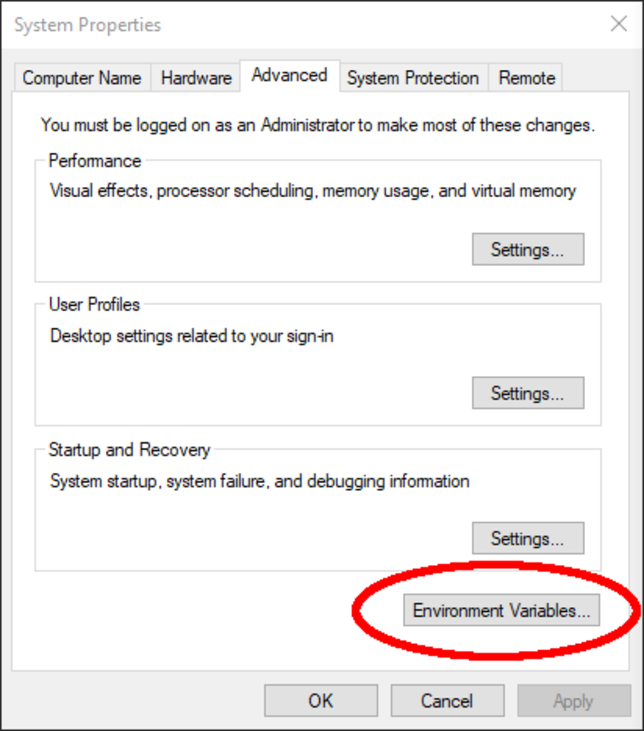
\includegraphics[width=\textwidth]{Figures/win/Win1.pdf}
(a)
\end{center}
\end{minipage}
\begin{minipage}[t]{.29\textwidth}
\begin{center}
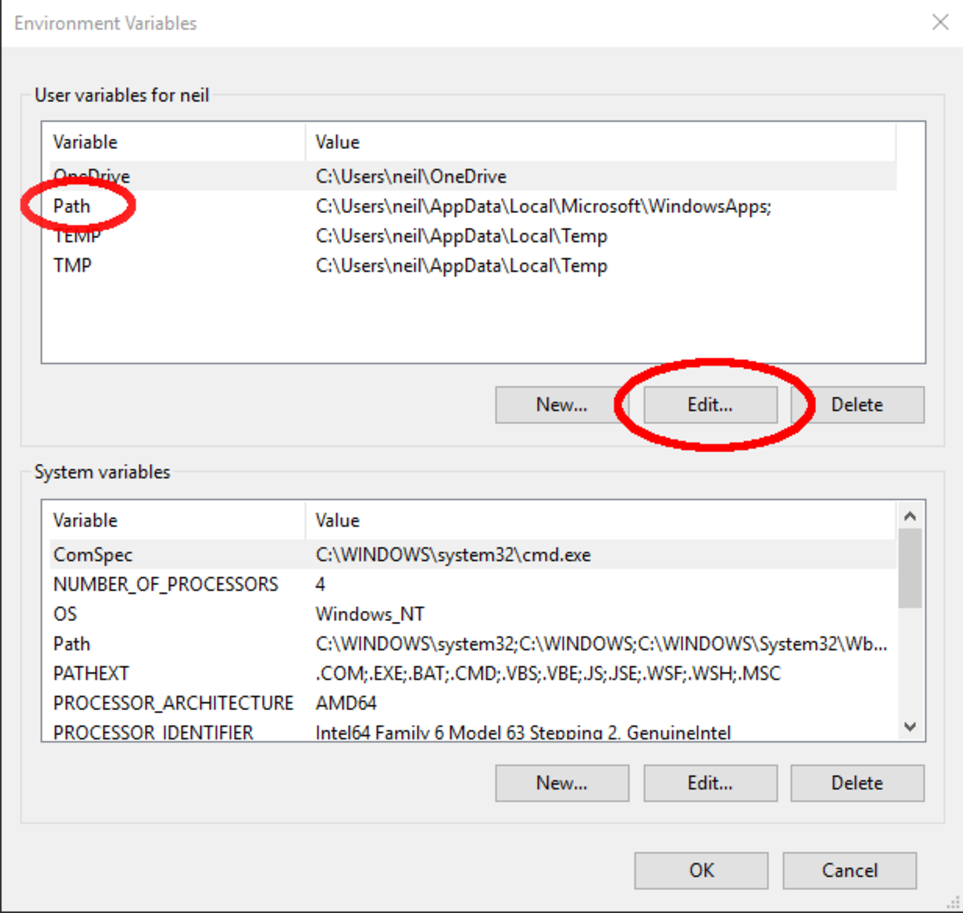
\includegraphics[width=\textwidth]{Figures/win/Win2.pdf}
(b)
\end{center}
\end{minipage}
\begin{minipage}[t]{.29\textwidth}
\begin{center}
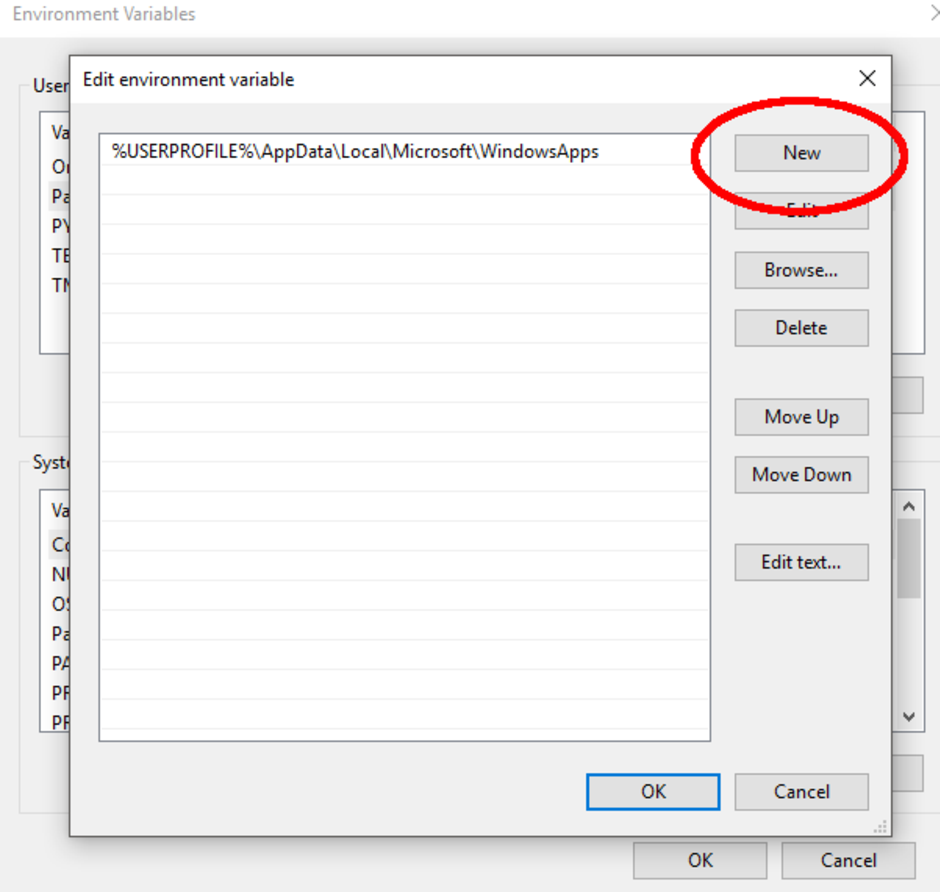
\includegraphics[width=\textwidth]{Figures/win/Win3.pdf}
(c)
\end{center}
\end{minipage}

\begin{minipage}[t]{.29\textwidth}
\begin{center}
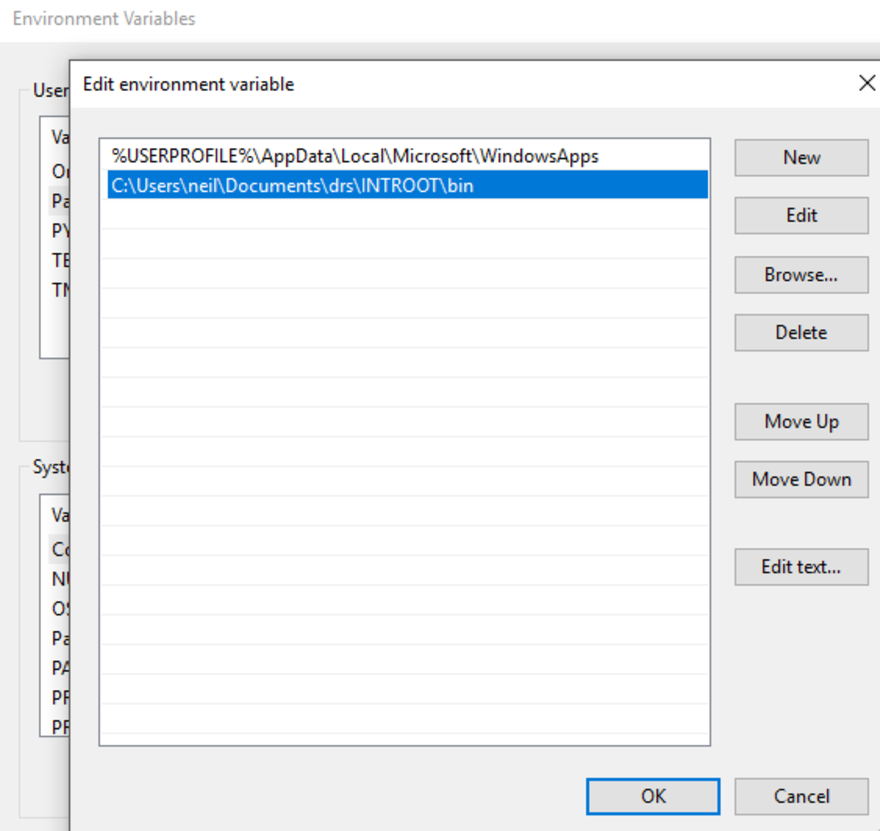
\includegraphics[width=\textwidth]{Figures/win/Win4.pdf}
(d)
\end{center}
\end{minipage}
\begin{minipage}[t]{.29\textwidth}
\begin{center}
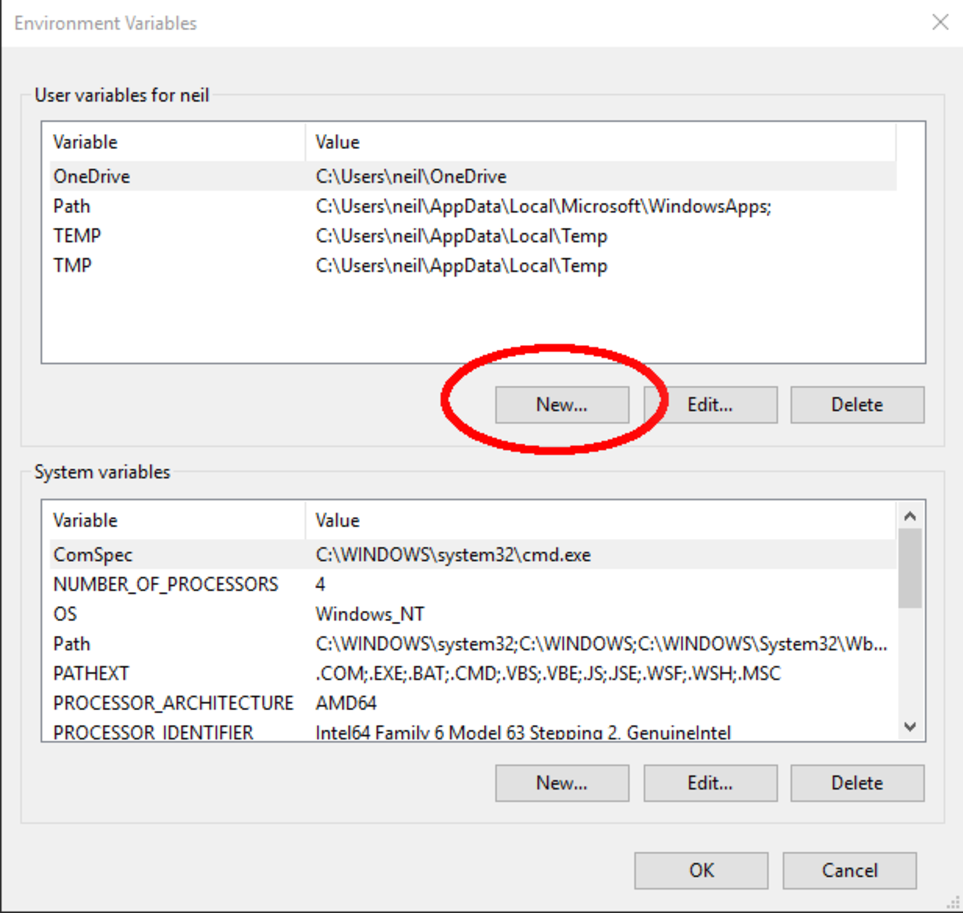
\includegraphics[width=\textwidth]{Figures/win/Win5.pdf}
(e)
\end{center}
\end{minipage}
\begin{minipage}[t]{.29\textwidth}
\begin{center}
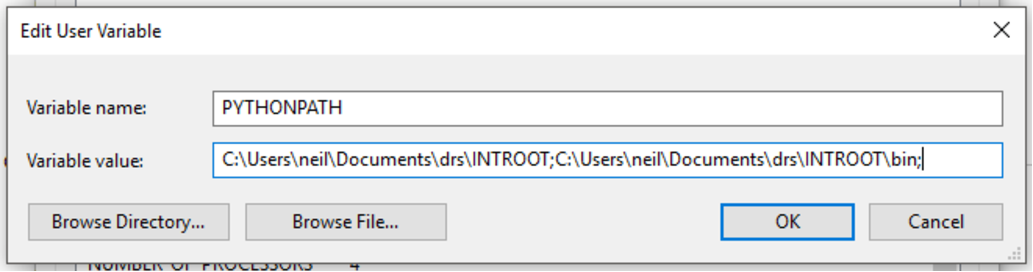
\includegraphics[width=\textwidth]{Figures/win/Win6.pdf}
(f)
\end{center}
\end{minipage}
\end{center}
\caption{(a) Once in ``Advanced system properties'' click ``Environment Variables'' (b) Click ``Path'' and click ``Edit...'' to edit the ``Path'' environmental variable (c) Once in the ``Path'' environmental variable click ``New'' to add a new path (d) Type in the new line to add variable and click ``OK'' (e) Once back in the Enivronmental variable page click ``New'' to add `PYTHONPATH' (f) Set the variable name to ``PYTHONPATH'' and edit the variable value accordingly. \label{figure:screengrabs} }
\end{figure}
\vspace{0.25cm}



%%%%%%%%%%%%%%%%%%%%%%%%%%%%%%%%%%%%%%%%%%%%%%%%%%%%%%%%
%%
\clearpage
\newpage
\section{Setting up the DRS (Windows)}
\label{ch:install:setup_win}
%%
%%%%%%%%%%%%%%%%%%%%%%%%%%%%%%%%%%%%%%%%%%%%%%%%%%%%%%%%

Before running the DRS one must set the data paths. \\

\noindent The `\configtxtfile' file is located in the \InstallDIR in the config folder.

i.e. at \InstallDIR\path{\\config\\}{configtxtfile} \\

\noindent The following keywords \textbf{must} be changed (and must be a valid path):
\begin{thighlight}
\begin{table}[H]
{\footnotesize
\begin{tabular}{p{4cm} p{0.05cm} p{2.5cm} p{0.05cm} p{5.5cm}}
\definevariable{text:drs_root}{TDATA}            & = & \path{C:\\Users\\User\\Documents\\drs\\data}        & / & Define the DATA directory\\
&&&&\\
\definevariable{text:drs_root}{DRS\_ROOT}         & = & \path{C:\\Users\\User\\Documents\\drs\\INTROOT}     & / & Define the installation directory \\
\definevariable{text:drs_data_raw}{DRS\_DATA\_RAW}     & = & \path{C:\\Users\\User\\Documents\\drs\\data\\raw}    & / & Define the folder with the raw data files in \\
\definevariable{text:drs_data_reduc}{DRS\_DATA\_REDUC}   & = & \path{C:\\Users\\User\\Documents\\drs\\data\\reduced} & / & Define the directory that the reduced data should be saved to/read from \\
\definevariable{text:drs_calib_db}{DRS\_CALIB\_DB}     & = & \path{C:\\Users\\User\\Documents\\drs\\data\\calibDB} & / & Define the directory that the calibration files should be saved to/read from \\
\definevariable{text:drs_data_msg}{DRS\_DATA\_MSG}     & = & \path{C:\\Users\\User\\Documents\\drs\\data\\msg}    & / & Define the directory that the log messages are stored in \\
\definevariable{text:drs_data_working}{DRS\_DATA\_WORKING} & = & \path{C:\\Users\\User\\Documents\\drs\\data\\tmp}    & / & Define the working directory \\
\end{tabular}
}
\end{table}
\end{thighlight}
\begin{note}
Note: On windows paths in windows must have a `\textbackslash\textbackslash' also the python files must be open with a valid editor such as sublime text, notepad++, spyder or pycharm for example
\end{note}

\vspace{0.25cm}

\noindent The following keywords can be changed: \\
\begin{thighlight}
\begin{table}[H]
\begin{tabular}{>{\color{red}}l c r c p{5cm}}
\definevariable{text:drs_plot}{DRS\_PLOT}    & = & 1     & / & Whether to show plots \\
\definevariable{text:print_level}{PRINT\_LEVEL} & = & "all" & / & Level at which to print \\
\definevariable{text:log_level}{LOG\_LEVEL}   & = & "all" & / & Level at which to log in log file \\
\end{tabular}
\end{table}

\noindent For the `\definevariable{text:print_level}{PRINT\_LEVEL} and \definevariable{text:log_level}{LOG\_LEVEL} keywords the values are set as follows:
\begin{itemize}
	\item "all" -- prints all events
	\item "info" -- prints info, warning and error events
	\item "warning" -- prints warning and error events
	\item "error" -- print only error events
\end{itemize}
\end{thighlight}



%%%%%%%%%%%%%%%%%%%%%%%%%%%%%%%%%%%%%%%%%%%%%%%%%%%%%%%%
%%
\clearpage
\newpage
\section{Validating Installation on Windows}
\label{ch:install:validating_installwin}
%%
%%%%%%%%%%%%%%%%%%%%%%%%%%%%%%%%%%%%%%%%%%%%%%%%%%%%%%%%

\begin{note}
One must install the DRS (Section \ref{ch:install:install_win}) AND set up the DRS (Section \ref{ch:install:setup}) before validation will be successful.
\end{note}

\noindent In windows there are currently 3 ways to run the RS (running in python/ipython).

\begin{itemize}
\item To validate running from python/ipython from the command line type:
\begin{cmdbox}
python (*\calvalidate*)
ipython (*\calvalidate*)
\end{cmdbox}

\item To validate running from ipython, open ipython and type:
\begin{pythonbox}
@run@ (*\calvalidate*)
\end{pythonbox}

\item To validate running from import from python/ipython, open python/ipython and type:
\begin{pythonbox}
import cal_validate_spirou
cal_validate_spirou.main()
\end{pythonbox}

\end{itemize}

\noindent If validation is successful the following should appear:
\begin{cmdboxprintspecial}
@g
17:34:19.0 -   || *****************************************
17:34:19.0 -   || * SPIROU @(#) Geneva Observatory (0.1.016)
17:34:19.0 -   || *****************************************
17:34:19.0 -   ||(dir_data_raw)      DRS_DATA_RAW=C:\\Users\\User\\Documents\\drs\\data\\raw
17:34:19.0 -   ||(dir_data_reduc)    DRS_DATA_REDUC=C:\\Users\\User\\Documents\\drs\\data\\reduced
17:34:19.0 -   ||(dir_calib_db)      DRS_CALIB_DB=C:\\Users\\User\\Documents\\drs\\data\\calibDB
17:34:19.0 -   ||(dir_data_msg)      DRS_DATA_MSG=C:\\Users\\User\\Documents\\drs\\data\\msg
17:34:19.0 -   ||(print_level)       PRINT_LEVEL=all         %(error/warning/info/all)
17:34:19.0 -   ||(log_level)         LOG_LEVEL=all         %(error/warning/info/all)
17:34:19.0 -   ||(plot_graph)        DRS_PLOT=1            %(def/undef/trigger)
17:34:19.0 -   ||(used_date)         DRS_USED_DATE=undefined
17:34:19.0 -   ||(working_dir)       DRS_DATA_WORKING=C:\\Users\\User\\Documents\\drs\\data\\tmp
17:34:19.0 -   ||                    DRS_INTERACTIVE is not set, running on-line mode
17:34:19.0 -   ||                    DRS_DEBUG is set, debug mode level:1
17:34:19.0 -   ||
17:34:19.0 -   ||Validation successful. DRS installed corrected.
@g
\end{cmdboxprintspecial}

% Chapter 2: Data Architecture
%%%%%%%%%%%%%%%%%%%%%%%%%%%%%%%%%%%%%%%%%%%%%%%%%%%%%%%%
%%
\chapter{Data Architecture}
\label{chapter:data_architecture}
%%
%%%%%%%%%%%%%%%%%%%%%%%%%%%%%%%%%%%%%%%%%%%%%%%%%%%%%%%%

% Chapter 3: Using the DRS
%%%%%%%%%%%%%%%%%%%%%%%%%%%%%%%%%%%%%%%%%%%%%%%%%%%%%%%%
%%
\chapter{Using the DRS}
\label{chapter:using_the_drs}
%%
%%%%%%%%%%%%%%%%%%%%%%%%%%%%%%%%%%%%%%%%%%%%%%%%%%%%%%%%

There are two ways to run the DRS recipes. The first (described in Section \ref{chapter:using_the_drs:direct}) directly calls the code and inputs arguments (either from the command line or from python), the second way is to import the recipes in a python script and define arguments in a call to a function (see Section \ref{chapter:using_the_drs:script}).

%%%%%%%%%%%%%%%%%%%%%%%%%%%%%%%%%%%%%%%%%%%%%%%%%%%%%%%%
%%
\section{Running the DRS recipes directly}
\label{chapter:using_the_drs:direct}
%%
%%%%%%%%%%%%%%%%%%%%%%%%%%%%%%%%%%%%%%%%%%%%%%%%%%%%%%%%

As in Chapter \ref{chapter:installation}, using Linux or \mac one can run DRS recipes from the command line or from python, in windows one is required to be in python before running the scipts. Below we use \calDARK as an example:
\begin{itemize}
\item To run from command line type:
\begin{cmdbox}
(*\calDARK*) YYMMDD Filenames
\end{cmdbox}

\item To run from python/ipython from the command line type:
\begin{cmdbox}
python (*\calDARK*) YYMMDD Filenames
ipython (*\calDARK*) YYMMDD Filenames
\end{cmdbox}

\item To run from ipython, open ipython and type:
\begin{pythonbox}
@run@ (*\calDARK*) YYMMDD Filenames
\end{pythonbox}
\end{itemize}

%%%%%%%%%%%%%%%%%%%%%%%%%%%%%%%%%%%%%%%%%%%%%%%%%%%%%%%%
%%
\section{Running the DRS recipes from a python script}
\label{chapter:using_the_drs:script}
%%
%%%%%%%%%%%%%%%%%%%%%%%%%%%%%%%%%%%%%%%%%%%%%%%%%%%%%%%%

In any operating system one can also import a recipe and call a function to run the code. This is useful in batch operations, timing tests and unit tests for example. Below we use \calDARK as an example:

\begin{pythonbox}
# import the recipe
import cal_DARK_spirou
# define the night folder name
night_name = "20170710"
# define the file(s) to run through the code
files = ['dark_dark02d406.fits']
# run code
cal_validate_spirou.main(night_name=night_name, files=files)
\end{pythonbox}


%%%%%%%%%%%%%%%%%%%%%%%%%%%%%%%%%%%%%%%%%%%%%%%%%%%%%%%%
%%
\section{Working example of the code for SPIRou}
\label{chapter:using_the_drs:working_example}
%%
%%%%%%%%%%%%%%%%%%%%%%%%%%%%%%%%%%%%%%%%%%%%%%%%%%%%%%%%

% ----------------------------------------------
\subsection{Overview}
\label{chapter:using_the_drs:working_example:overview}
% ----------------------------------------------

For this example all files are from:
\begin{cmdbox}
spirou@10.102.14.81:/data/RawImages/H2RG-AT4/AT4-04/2017-07-10_15-36-18/ramps/
\end{cmdbox} 

\noindent following our example data architecture (from Section \ref{ch:install:setup} and shown explicity in Section \ref{ch:data_architecture:folder_layout}) all files should be places in the \definevariable{text:drs_data_raw}{DRS\_DATA\_RAW} (\textcolor{blue}{/drs/data/raw} in our case).

\noindent and we will also need the current WAVE file from here:
\begin{cmdbox}
spirou@10.102.14.81:/data/reduced/DATA-CALIB/spirou_wave_ini3.fits
\end{cmdbox}

\noindent which needs to be placed in the \definevariable{text:drs_calib_db}{DRS\_CALIB\_DB} dirctory (\textcolor{blue}{/drs/data/calibDB} in our case).

\noindent Starting with RAMP files and ending with extracted orders and calculated drifts we need to run six codes:
\begin{enumerate}
\item \calDARK \hfill (See Section \ref{ch:the_recipes:cal_DARK_spirou})
\item \callocRAW ($\times$2) \hfill (See Section \ref{ch:the_recipes:cal_loc_RAW_spirou})
\item \calSLIT \hfill (See Section \ref{ch:the_recipes:cal_SLIT_spirou})
\item \calFFraw ($\times$2) \hfill (See Section \ref{ch:the_recipes:cal_FF_RAW_spirou})
\item (add spirou\_wave\_ini3.fits to calibDB) 
\item \calextractRAWAB and \calextractRAWC (many times) \hfill (See Section \ref{ch:the_recipes:cal_extract_RAW_spirou})
\item \calDRIFTRAW \hfill (See Section \ref{ch:the_recipes:cal_DRIFT_RAW_spirou})
\end{enumerate}





% ----------------------------------------------
\subsection{Run through from command line/python shell (Linux and macOS)}
\label{chapter:using_the_drs:working_example:run_cmd}
% ----------------------------------------------

As long as all codes are excutable (see Section \ref{ch:install:installunix:executable}) one can run all codes from the command line or if not excutable or one has a preference for python one can run the following with `python \{command\}', `ipython \{command\}' or indeed through an interactive ipython session using `run \{command\}'.

\begin{enumerate}

\item run the dark extraction on the `dark\_dark' file:
\begin{cmdbox}
cal_DARK_spirou.py 20170710 dark_dark02d406.fits
\end{cmdbox}

\item run the order localisation on the `dark\_flat' files:
\begin{cmdbox}
cal_loc_RAW_spirou.py 20170710 dark_flat02f10.fits dark_flat03f10.fits dark_flat04f10.fits dark_flat05f10.fits dark_flat06f10.fits
\end{cmdbox}

\item run the order localisation on the `flat\_dark' files:
\begin{cmdbox}
cal_loc_RAW_spirou.py 20170710 flat_dark02f10.fits flat_dark03f10.fits flat_dark04f10.fits flat_dark05f10.fits flat_dark06f10.fits
\end{cmdbox}

\item run the slit calibration on the `fp\_fp' files.
\begin{cmdbox}
cal_SLIT_spirou.py 20170710 fp_fp02a203.fits fp_fp03a203.fits fp_fp04a203.fits
\end{cmdbox}

\item run the flat field creation on the `dark\_flat' files:

\begin{note}
if using same files as above you will get an error message when running the file.

\noindent To solve this open the `\masterCALIBDBfile' file located in \textcolor{blue}{\{DATA\_ROOT\_CALIB\}}. Edit the unix date in the line that begins `TILT' so that it is less than or equal to the unix date on rows `ORDER\_PROFIL\_AB' (i.e. easiest to change it to the date on the `ORDER\_PROFIL\_AB')

\noindent The human date format must match the unix date thus both must be changed if one is modified.

\noindent i.e. the `\masterCALIBDBfile' file should look go from
\begin{textbox}
DARK 20170710 dark_dark02d406.fits 07/10/17/16:37:48 1499704668.0
ORDER_PROFIL_C 20170710 dark_flat02f10_order_profil_C.fits 07/10/17/17:03:50 1499706230.0
LOC_C 20170710 dark_flat02f10_loco_C.fits 07/10/17/17:03:50 1499706230.0
ORDER_PROFIL_AB 20170710 flat_dark02f10_order_profil_AB.fits 07/10/17/17:07:08 1499706428.0
LOC_AB 20170710 flat_dark02f10_loco_AB.fits 07/10/17/17:07:08 1499706428.0
TILT 20170710 fp_fp02a203_tilt.fits @07/10/17/17:25:15 1499707515.0@
\end{textbox}
\noindent to this:
\begin{textbox}
DARK 20170710 dark_dark02d406.fits 07/10/17/16:37:48 1499704668.0
ORDER_PROFIL_C 20170710 dark_flat02f10_order_profil_C.fits 07/10/17/17:03:50 1499706230.0
LOC_C 20170710 dark_flat02f10_loco_C.fits 07/10/17/17:03:50 1499706230.0
ORDER_PROFIL_AB 20170710 flat_dark02f10_order_profil_AB.fits 07/10/17/17:07:08 1499706428.0
LOC_AB 20170710 flat_dark02f10_loco_AB.fits 07/10/17/17:07:08 1499706428.0
TILT 20170710 fp_fp02a203_tilt.fits @07/10/17/17:07:08 1499706428.0@
\end{textbox}
\end{note}

\begin{cmdbox}
cal_FF_RAW_spirou.py 20170710 dark_flat02f10.fits dark_flat03f10.fits dark_flat04f10.fits dark_flat05f10.fits dark_flat06f10.fits
\end{cmdbox}

\newpage

\item Currently we do not create a new wavelength calibration file for this run. Therefore we need one (as stated in the above section). We use the one from here:
\begin{cmdbox}
spirou@10.102.14.81:/data/reduced/DATA-CALIB/spirou_wave_ini3.fits
\end{cmdbox}

\noindent then place it in the \definevariable{text:drs_calib_db}{DRS\_CALIB\_DB} folder. You will also need to edit the `\masterCALIBDBfile' file located in \definevariable{text:drs_calib_db}{DRS\_CALIB\_DB}. 

\noindent Add the folloing line to `\masterCALIBDBfile'
\begin{textbox}
@WAVE 20170710 spirou_wave_ini3.fits 07/10/17/17:03:50 1499706230.0@
\end{textbox}

\noindent and the `master\_calib\_SPIROU.txt' should look like this:
\begin{textbox}
DARK 20170710 dark_dark02d406.fits 07/10/17/16:37:48 1499704668.0
ORDER_PROFIL_C 20170710 dark_flat02f10_order_profil_C.fits 07/10/17/17:03:50 1499706230.0
LOC_C 20170710 dark_flat02f10_loco_C.fits 07/10/17/17:03:50 1499706230.0
ORDER_PROFIL_AB 20170710 flat_dark02f10_order_profil_AB.fits 07/10/17/17:07:08 1499706428.0
LOC_AB 20170710 flat_dark02f10_loco_AB.fits 07/10/17/17:07:08 1499706428.0
TILT 20170710 fp_fp02a203_tilt.fits 07/10/17/17:07:08 1499706428.0
@WAVE 20170710 spirou_wave_ini3.fits 07/10/17/17:03:50 1499706230.0@
\end{textbox}

\item run the extraction files on the `hcone\_dark', `dark\_hcone', `hcone\_hcone', `dark\_dark\_AHC1', `hctwo\_dark', `dark\_hctwo', `hctwo-hctwo', `dark\_dark\_AHC2' and `fp\_fp'  files. For example for the `fp\_fp' files:
\begin{cmdbox}
cal_extract_RAW_spirouAB.py 20170710 fp_fp02a203.fits fp_fp03a203.fits fp_fp04a203.fits
cal_extract_RAW_spirouC.py 20170710 fp_fp02a203.fits fp_fp03a203.fits fp_fp04a203.fits
\end{cmdbox}

\item run the drift calculation on the `fp\_fp' files:
\begin{cmdbox}
@cal_DRIFT_RAW_spirou.py 20170710 @fp_fp02a203.fits fp_fp03a203.fits fp_fp04a203.fits
\end{cmdbox}

\end{enumerate}

% ----------------------------------------------
\clearpage
\newpage
\subsection{Run through python script}
\label{chapter:using_the_drs:working_example:run_python}
% ----------------------------------------------

The process is in the same order as Section \ref{chapter:using_the_drs:working_example:run_cmd}, including changing the date on the `TILT' keyword and adding the `WAVE' line, and adding the wave file to the calibDB folder).

\begin{pythonbox}
import cal_DARK_spirou, cal_loc_RAW_spirou
import cal_SLIT_spirou, cal_FF_RAW_spirou
import cal_extract_RAW_spirou, cal_DRIFT_RAW_spirou
import matplotlib.pyplot as plt
# define constants
NIGHT_NAME = '20170710'
# cal_dark_spirou
files = ['dark_dark02d406.fits']          # set up files
cal_DARK_spirou.main(NIGHT_NAME, files)   # run cal_dark_spirou
plt.close('all')                          # close graphs
# cal_loc_RAW_spirou - flat_dark
files = ['flat_dark02f10.fits', 'flat_dark03f10.fits', 'flat_dark04f10.fits',
         'flat_dark05f10.fits','flat_dark06f10.fits']
cal_loc_RAW_spirou.main(NIGHT_NAME, files)
plt.close('all')
# cal_loc_RAW_spirou - dark_flat
files = ['dark_flat02f10.fits', 'dark_flat03f10.fits', 'dark_flat04f10.fits', 
         'dark_flat05f10.fits', 'dark_flat06f10.fits']
cal_loc_RAW_spirou.main(NIGHT_NAME, files)
plt.close('all')
# cal_SLIT_spirou
files = ['fp_fp02a203.fits', 'fp_fp03a203.fits', 'fp_fp04a203.fits']
cal_SLIT_spirou.main(NIGHT_NAME, files)
plt.close('all')
# cal_FF_RAW_spirou - flat_dark
files = ['flat_dark02f10.fits', 'flat_dark03f10.fits','flat_dark04f10.fits',
         'flat_dark05f10.fits', 'flat_dark06f10.fits']
cal_FF_RAW_spirou.main(NIGHT_NAME, files)
plt.close('all')
# cal_FF_RAW_spirou - dark_flat
files = ['dark_flat02f10.fits', 'dark_flat03f10.fits', 'dark_flat04f10.fits', 
         'dark_flat05f10.fits', 'dark_flat06f10.fits']
cal_FF_RAW_spirou.main(NIGHT_NAME, files)
plt.close('all')
# cal_extract_RAW_spirou - fp_fp AB
files = ['fp_fp02a203.fits', 'fp_fp03a203.fits', 'fp_fp04a203.fits']
cal_extract_RAW_spirou.main(NIGHT_NAME, files, 'AB')
plt.close('all')
# cal_extract_RAW_spirou - fp_fp C
files = ['fp_fp02a203.fits', 'fp_fp03a203.fits', 'fp_fp04a203.fits']
cal_extract_RAW_spirou.main(NIGHT_NAME, files, 'C')
plt.close('all')
# test cal_DRIFT_RAW_spirou
files = ['fp_fp02a203.fits', 'fp_fp03a203.fits', 'fp_fp04a203.fits']
cal_DRIFT_RAW_spirou.main(NIGHT_NAME, files)
plt.close('all')

\end{pythonbox}


% Chapter 4: User Modifiable Variables
%%%%%%%%%%%%%%%%%%%%%%%%%%%%%%%%%%%%%%%%%%%%%%%%%%%%%%%%
%%
\chapter{User modifiable variables}
\label{chapter:user_mod_variables}
%%
%%%%%%%%%%%%%%%%%%%%%%%%%%%%%%%%%%%%%%%%%%%%%%%%%%%%%%%%

% Chapter 5: The Recipes
%%%%%%%%%%%%%%%%%%%%%%%%%%%%%%%%%%%%%%%%%%%%%%%%%%%%%%%%
%%
\chapter{The Recipes}
\label{chapter:the_recipes}
%%
%%%%%%%%%%%%%%%%%%%%%%%%%%%%%%%%%%%%%%%%%%%%%%%%%%%%%%%%

% % Appendi
% \appendix

% % \addtocontents{toc}{\setlength\cftchapternumwidth{1em}}

% % Appendix A: env_setup.sh
% \input{Chapters/appendix_env_setup_sh}

%%%-------------------------------------------------------------------------------

\backmatter

%%% BIBLIOGRAPHY
%%% -------------------------------------------------------------

% \bibliographystyle{utphysics}
% \bibliography{ref}

\end{document}
